\documentclass[border=10pt]{standalone}
\usepackage{pgfplots}
\usetikzlibrary{arrows.meta, shapes, calc}
\pgfplotsset{compat=1.18}

\begin{document}
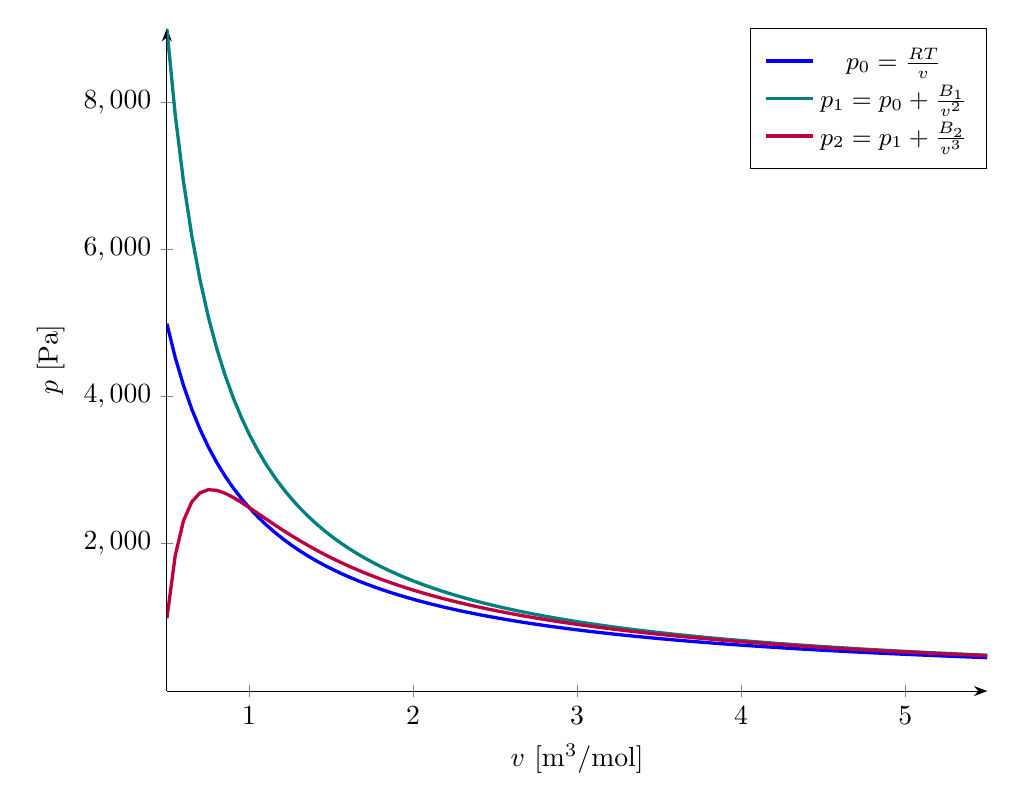
\begin{tikzpicture}
\begin{axis}[
    axis lines = left,
    axis line style={-Stealth},
    xlabel = {$v$ [m$^3$/mol]},
    ylabel = {$p$ [Pa]},
    xmin=0.5, xmax=5.5,
    ymin=0, ymax=9000,
    xtick={1,2,3,4,5},
    ytick={2000,4000,6000,8000},
    scaled y ticks=false,
    yticklabel style={/pgf/number format/fixed, /pgf/number format/1000 sep={,}},
    legend style={
        at={(1,1)},
        anchor=north east,
        draw=black,
        fill=white,
        inner sep=5pt,
        font=\small
    },
    width=12cm,
    height=10cm,
    every axis plot/.append style={very thick},
]

% p0 = RT/v
\addplot[blue, domain=0.5:5.5, samples=100] {8.314462618 * 300 / x};
\addlegendentry{$p_0 = \frac{R T}{v}$}

% p1 = p0 + B1/v^2
\addplot[teal, domain=0.5:5.5, samples=100] {8.314462618 * 300 / x + 1000 / (x^2)};
\addlegendentry{$p_1 = p_0 + \frac{B_1}{v^2}$}

% p2 = p1 + B2/v^3
\addplot[purple, domain=0.5:5.5, samples=100] {8.314462618 * 300 / x + 1000 / (x^2) - 1000 / (x^3)};
\addlegendentry{$p_2 = p_1 + \frac{B_2}{v^3}$}

\end{axis}
\end{tikzpicture}
\end{document}
